\documentclass[]{article}

\usepackage{geometry}
\geometry{textwidth = 18cm,textheight = 24cm}

\usepackage{multicol}
\usepackage{cite}
\usepackage{caption}
\usepackage{graphicx}
\usepackage{amsmath}
\usepackage{amssymb}
\usepackage{textcomp}
\usepackage{lmodern}
\usepackage{authblk}

\newcommand{\onlinecite}[1]{\hspace{-1 ex} \nocite{#1}\citenum{#1}} 

\newenvironment{Figure}
  {\par\medskip\noindent\minipage{\linewidth}}
  {\endminipage\par\medskip}


\begin{document}
    
\begin{center}
\LARGE{Phenomenological modeling of loop neurons}\\ 
\vspace{0.3em}
\large From: Jeff Shainline \\
\large To: Andrew Dienstfrey\\
\vspace{0.0em}
\textit{\small National Institute of Standards and Technology, Boulder, CO, 80305}\\
\vspace{0.3em}
\small \today

\begin{abstract}

\vspace{1em}
\end{abstract}

\end{center}

%\begin{multicols}{2}

\setcounter{tocdepth}{1}
\setcounter{secnumdepth}{4}
\tableofcontents

\section{\label{sec:introduction}Introduction}
The purpose of the present document is to communicate to you, Andrew Dienstrfrey, a few concepts regarding the circuits we are exploring so that you can help me construct a set of phenomenological models that will enable numerical investigation of these circuits as synapses, dendrites, neurons, and networks. I think the phenomenological model is the best way for me to communicate with you and provide you with the tools you need to think about this work. This document in its present form is basically just a set of notes that I hope to use to further the conversation you and I had in your office on June 19th, 2019. There are many exciting avenues to pursue that I think will be facilitated by an efficient numerical implementation of the models presented here, and I would benefit immensely from your insights when proceeding to numerically investigate more complex systems. The avenues of excitement are discussed in Sec.\,\ref{sec:future_directions}. First, I include a qualitative description of loop neuron operation before discussing the model.

\section{\label{sec:qualitative_explanation_of_loop_neurons}Qualitative Explanation of Loop Neurons}
\begin{figure}
\centering
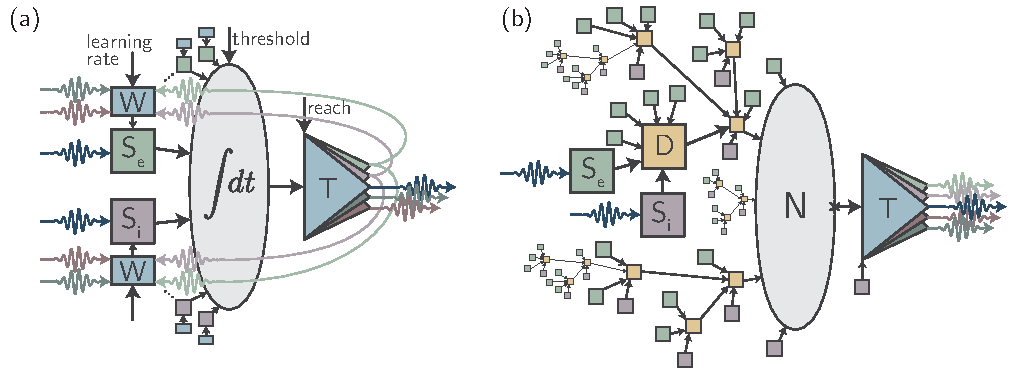
\includegraphics[width=17.2cm]{_01__schematic.pdf}
\captionof{figure}{\label{fig:schematic}Two schematics of loop neurons. (a) A point loop neuron (no dendritic tree) showing excitatory ($\mathsf{S_e}$) and inhibitory ($\mathsf{S_i}$) synapses, as well as synaptic weight update circuits ($\mathsf{W}$). The wavy, colored arrows are photons, and the straight, black arrows are electrical signals. The synapses receive signals as faint as a single photon and add supercurrent to an integration loop. Upon reaching threshold, a signal is sent to the transmitter circuit ($\mathsf{T}$), which produces a photon pulse. Some photons from the pulse are sent to downstream synaptic connections, while some are used locally to update synaptic weights. (b) A loop neuron with an elaborate dendritic tree. The complex structure consists of excitatory and inhibitory synapses that feed into dendrites ($\mathsf{D}$). Each dendrite performs computations on the inputs and communicates the result to other dendrites for further processing or on to the cell body of the neuron ($\mathsf{N}$). The neuron itself acts as the final thresholding stage, and when its threshold is reached, light is produced by the transmitter ($\mathsf{T}$), which is routed to downstream synaptic connections.}
\end{figure}
Schematic diagrams of two types of loop neuron are shown in Fig.\,\ref{fig:schematic}. Figure \ref{fig:schematic}(a) shows the point-neuron concept \cite{sh2018,sh2019_jap}, while Fig.\,\ref{fig:schematic}(b) shows the concept when a dendritic tree is included \cite{sh2019_jstqe}. In these neurons, integration, synaptic plasticity, and dendritic processing are implemented with inductively coupled loops of supercurrent. It is due to the prominent role of superconducting storage loops that we refer to devices of this type as loop neurons. Operation is as follows. Photons from upstream neurons are received by a superconducting single-photon detectors (SPD) at each synapse. Using a Josephson junction (JJ) in parallel with an SPD, synaptic detection events are converted into an integrated supercurrent which is stored in a superconducting loop. The circuit diagram of a synapse is shown in Fig.\,\ref{fig:circuits}(a). The amount of current that gets added to the integration loop during a photon detection event is determined by the synaptic weight. The synaptic weight is dynamically adjusted by another circuit combining SPDs and JJs, and all involved circuits are analog. When the integrated current of a given neuron reaches a (dynamically variable) threshold, an amplification cascade begins, resulting in the production of light from a waveguide-integrated semiconductor light emitter. The amplifer and it use in the production of light is experimentally demonstrated in Ref.\,\onlinecite{mcve2019}. The photons thus produced fan out through a network of dielectric waveguides and arrive at the synaptic terminals of other neurons where the process repeats. We have described and demonstrated these networks of multiplanar waveguides in Refs.\,\onlinecite{chbu2017} and \onlinecite{chbu2018}. We demonstrated the silicon light sources waveguide-integrated with superconducting single-photon detectors in Ref.\,\onlinecite{buch2017}.

\begin{figure}
\centering
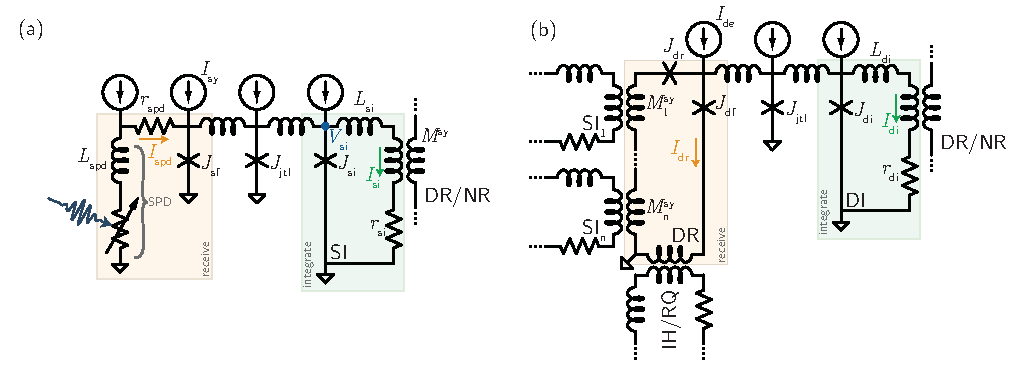
\includegraphics[width=17.2cm]{_02__circuits.pdf}
\captionof{figure}{\label{fig:circuits}Circuit diagrams. (a) A synapse combining a single-photon detector (SPD) in parallel with a Josephson junction (JJ). The generated signal is stored in the synaptic integration (SI) loop. (b) A dendrite using a similar circuit structure to (a) to perform nonlinear functions on multiple synaptic or dendritic inputs. The inputs are received by the dendritic receiving (DR) loop and, the outputs are stored in the dendritic integration (DI) loop. Inhibitory inputs (IH) can also be utilized.}
\end{figure}

In loop neurons, a synapse consists of an SPD in parallel with a JJ (which together transduce photons to supercurrent), and a superconducting loop, which stores a current proportional to the number of detected photon arrival events. This loop is referred to as the synaptic integration (SI) loop. Within each neuron, the loops of many synapses are inductively coupled to a larger superconducting loop, referred to as the neuronal receiving (NR) loop, thereby inducing an integrated current proportional to a weighted sum of the currents in all the neuron's synapses. When the current in this NI loop reaches a threshold, the neuron produces a current pulse in the form of one or more flux quanta. This current is amplified and converted to voltage to produce photons from a semiconductor $p-i-n$ junction.

The currents in the synaptic and neuronal loops are analogous to the membrane potential of biological neurons \cite{daab2001,geki2002}, and the states of flux in these loops are the principal dynamical variables of the synapses and neurons in the system. Inhibitory synapses can be achieved through mutual inductors with the opposite sign of coupling. Dendritic processing can be implemented straightforwardly by adding intermediate mutually inductively coupled loops between the synaptic and neuronal loops. Synapses can be grouped on dendritic loops capable of local, nonlinear processing and inhibition. Neurons with multiple levels of dendritic hierarchy can be implemented as multiple stages of integrating loops. The temporal scales of the SI and DI loops can be set with $L/r$ time constants. I expect all synaptic and dendritic signals to leak, enabling fading memory of recent activity. Also, I hypothesize that the ability to achieve a diversity of time constants through synapses and dendrites with many $L/r$ time constants will be advantageous, and I would like to investigate this in numerical studies.

Synaptic memory is also implemented based on the stored flux in a loop, referred to as the synaptic storage (SS) loop. The state of flux in the SS loop determines the current bias to the synaptic receiver circuit discussed above. This current bias is the synaptic weight. In contrast to the SI and DI loops, the SS loop is intended to store long-term memory, and therefore I do not expect to add a resistance to this loop. If the SS loop is created with a superconducting wire of high inductance, the loop can hold many discrete states of flux, and therefore can implement many synaptic weights, if desired. Synapses with a pseudo-continuum of hundreds of stable synaptic levels between minimal and maximal saturation values are possible. Transitions between these levels can be induced based on the relative arrival times of photons from the pre-synaptic and post-synaptic neurons, thereby establishing a means for spike-timing-dependent plasticity with one photon required for each step of the memory-update process \cite{sh2019_jap}. Binary synapses are also possible, and just as we expect a diversity of $L/r$ time constants to be advantageous for tracking activity over time, we expect a diversity of synapses raging from binary to multistable to be advantageous for striking a balance between adaptability and stability.

\section{\label{sec:leaky_integrators}Leaky Integrators}
At this point, I think a good model of loop neurons with a dendritic tree involves a combination of two models: a leaky integrator model for dendrites and a spike response model for synapses. To make sure we're on the same page, here is a the way I think about these two models. A leaky integrator obeys the equation
\begin{equation}
\label{eq:leaky_integrator}
\frac{du(t)}{dt} = f_{\mathrm{in}}(t)-\tau^{-1}u(t).
\end{equation}
The function $f_{\mathrm{in}}(t)$ represents an arbitrary, time-varying input to the integrator, and $\tau$ gives the leak rate. The leaky integrate-and-fire model (I\&F) treats a system that follows Eq.\,\ref{eq:leaky_integrator}, but is also subject to the rule that when $u(t)$ reaches a threshold $\theta$, the system produces a pulse (spike, action potential, firing event), and the value of $u(t)$ is set to a base value $u_0$. Loop neurons can be made to behave exactly as leaky integrate-and-fire neurons in some circumstances, but I think they can perform better. In particular, the reset of $u$ after a firing event erases all information known to the neuron, and this seems wasteful.  

\section{\label{sec:spike_response_model}The Spike Response Model}
The spike response model (SRM) is a phenomenological model of neuron behavior that is complimentary to integrate-and-fire models. The approach leverages closed-form expressions for the response of the membrane potential to synaptic activity and production of action potentials. We can construct similar models based on loop neuron circuits to facilitate numerical analysis of loop neurons and networks.

I have only learned about SRM from the textbook called Spiking Neuron Models by Gerstner and Kistler \cite{geki2002}. From Gerstner and Kistler, pg. 102, the SRM is structured as follows. The state of neuron $i$ at time $t$ is described by a single variable, $u_i(t)$. In the absence of spikes, $u_i(t) = u_{\mathrm{rest}}$. The function
\begin{equation}
\label{eq:synaptic_response_kernel}
\epsilon_{ij}(t-t_j^{(f)})
\end{equation}
describes the time course of the response to an incoming spike train. The function $\epsilon$ is referred to as the \textit{synaptic response kernel}, and $t_j^{(f)}$ is the full list of times at which a pulse leaving neuron $j$ was received at a synapse on neuron $i$. If $u_i(t)$ reaches threshold $\theta$, an output spike is triggered. The response of the variable $u_i(t)$ to the production of this action potential is modeled by the function
\begin{equation}
\label{eq:reset_kernel}
\eta(t-\hat{t}_i),
\end{equation}
where $\hat{t}_i$ is the time of the last action potential produced by neuron $i$. The function $\eta$ is referred to as the \textit{reset kernel}. After firing, the evolution of $u_i(t)$ follows
\begin{equation}
\label{eq:spike_response_model}
u_i(t) = \eta(t-\hat{t}_i)+\sum_j w_{ij}\sum_f \epsilon_{ij}(t-t_j^{(f)}).
\end{equation}
In biological neurons, $\epsilon$ may also depend on $\hat{t}_i$ due to physiological activity with the cell due to action potential creation. Such behavior is not native to loop neurons. It could be added if advantageous, but at present we neglect it from the model. The time between when neuron $j$ produces a pulse and when it is received by neuron $i$ is the delay, and we neglect delay in this work. One can also include a term to account for external drive that takes the form
\begin{equation}
\label{eq:external_drive}
\int_0^{\infty}\kappa(t-\hat{t}_i,s)I^{\mathrm{ext}}(t-s)ds,
\end{equation}
but we also ignore this term and assume all external drives are input through synapses with response given by $\epsilon$.

For the purpose at hand, we consider Eq.\,\ref{eq:spike_response_model} to represent the SRM for point neurons in a form that is most relevant to modeling loop neurons.

\section{\label{sec:synapses}Phenomenological Model of Synapses}
In loop neurons, the best model for the neuron as a whole may not be a leaky integrator, but rather a spike response model for each synapse, a leaky integrator ODE for each dendrite, and a summation for the signal present in the neuron. Let us begin to model loop neurons by modeling a synapse in isolation. Let us first consider a synapse in the context of a leaky integration model and proceed from there to reduce it to a closed-form expression for the synaptic response to a firing event. 

In the circuit of Fig.\,\ref{fig:circuits}(a), the dynamical quantity that passes information to the rest of the neuron is the current circulating in the SI loop, $I_{\mathrm{si}}(t)$. Current is added to the loop when the synaptic firing junction, $J_{sf}$, is driven above the junction's critical current ($I_c$) by the redirection of current from the SPD to $J_{sf}$ during a synaptic firing event. Due to the nature of JJs, exceeding the $I_c$ of the junction results in the production of a series of fluxons. These fluxons are generated at a rate that is dependent on both the $I_c$ (which is static) and the current bias, $I_b$. The functional form of this current-dependent rate is not simple, in general, so we simply refer to the rate of production of flux quanta as $r_{fq}(I_b;t)$\footnote{In the case of junctions with damping parameter $\beta_c\ll 1$, there is a closed form expression: $r_{fq} = R\sqrt{I_b^2-I_c^2}$ for $I_b > I_c$, and zero otherwise. The damping parameter is $\beta_c = 2eI_cCR^2/\hbar$, where $C$ and $R$ are the junction capacitance and resistance.}. Each flux quantum that enters the SI loop adds a fixed amount of current to the loop, governed by the relation $\Delta I_{si} = \Phi_0/L_{si}$, where $\Phi_{0} = h/2e = 2.07\times 10^{-15}$\,Wb is the magnetic flux quantum, and $L_{si}$ is the inductance of the SI loop. This relation between the current associated with a single fluxon and the inductance of the loop is a fundamental aspect of Josephson physics. The rate at which current is added to the SI loop equals the rate at which fluxons are generated multiplied by the current added to the loop with each fluxon. The current leaks exponentially from the SI loop with the time constant $\tau_{si} = L_{si}/r_{si}$. Thus, the current in the SI loop obeys a leaky integrator equation:
\begin{equation}
\label{eq:leaky_integrator__SI_loop}
\frac{dI_{si}(t)}{dt} = \alpha r_{fq}(I_b,t)-\tau_{si}^{-1}I_{si}(t).
\end{equation}
Here we expect $\alpha = \Phi_0/L_{si}$, but it can be considered simply a scale factor mapping input rate to current. Also, though current is added to the SI loop in increments of discrete flux quanta, we are dealing with pretty large numbers of flux quanta (10-1000 per synaptic firing event), so treating $r_{fq}$ as a continuous function is probably acceptable.

Based on this model, we can reduce all synaptic activity to the solution of first-order ODEs if we know $r_{fq}$ and the complete list of arrival times, $\bar{t}$. But in certain contexts it would be advantageous if we could avoid solving ODEs and instead simply write down the form of the response.

After some contemplation, we arrive at the expression
\begin{equation}
\label{eq:I_si}
I_{si}(\bar{t};t) = \sum_{q: t>t_{q}} f[I_{si}(t_{q})]\phantom{a}g[t-t_q,I_{si}(t_{q})]\phantom{a}e^{-(t-t_{q})/\tau_{si}},
\end{equation}
where $\bar{t}$ is the set of all firing times, $\bar{t} = \{t_q\}$, and $\tau_{si}$ is the $L/r$ leak rate of the SI loop chosen in design, set in hardware, and can be different for each synapse. In this summation, the notation $q:t>t_q$ refers to the fact that we are summing over synaptic firing events, and terms in the sum should not contribute at times before the time of the associated firing event. Equation \ref{eq:I_si} depends on the prefactor $f[I_{si}(t_q)]$ that depends on the value of $I_{si}$ at the time of the synaptic firing event:
\begin{equation}
\label{eq:I_si__prefactor}
f[I_{si}(t_q)] = \mathrm{min}\bigg(I_0\bigg[1-\bigg(\frac{I_{si}(t_q)}{I_{si}^{sat}}\bigg)^{\gamma_1}\bigg]^{\gamma_2},I_{si}^{sat}-I_{si}(t_q)\bigg).
\end{equation}
Equation \ref{eq:I_si} also depends on the rising term
\begin{equation}
\label{eq:I_si__rising_term}
g[t-t_q,I_{si}(t_q)]= 
\begin{cases}
   \bigg(\frac{t-t_q}{\tau_+}\bigg)^{\gamma_3} & \text{for }t-t_q<\tau_+\text{,}\\
    1              & \text{otherwise.}
\end{cases}
\end{equation}
Equation \ref{eq:I_si} with the prefactor of Eq.\,\ref{eq:I_si__prefactor} and the rising term of Eq.\,\ref{eq:I_si__rising_term} provide an accurate model of the synaptic response to an arbitrary pulse sequence specified by $\bar{t}$. These equations have three exponents, $\gamma_1$, $\gamma_2$, and $\gamma_3$. These have been determined from numerical experiments, and the values of $\gamma_1 = 0.9$, $\gamma_2 = 0.158$, and $\gamma_3 = 3/4$ achieve good fits to circuit models over a broad range of operating conditions. We can treat these exponents as known constants. The model also depends on two other factors: $I_0$ and $\tau_+$. These two factors both depend on the synaptic current bias (and therefore the synaptic weight), and should more appropriately be written $I_0[I_{sy}(t_q)]$ and $\tau_+[I_{sy}(t_q)]$. 

In the model of Eqs.\,\ref{eq:I_si} and \ref{eq:I_si__prefactor} we have come up with the form of the synaptic response kernel. Namely, 
\begin{equation}
\label{eq:I_si__synaptic_response_kernel}
\epsilon(\bar{t};t) \propto I_{si}(\bar{t};t).
\end{equation}
This is the spike response model of loop neuron synapses. Before showing how to employ this in the context of a neuron, we first consider the accuracy of the model in capturing the behavior of the circuits under consideration. We can accomplish this by comparing the model to circuits simulated with WRSpice.

(Insert relevant figs. here)

\section{\label{sec:neurons}Phenomenological Model of Point Neurons}
We have a closed-form expression (Eqs.\,\ref{eq:I_si} and \ref{eq:I_si__prefactor}) for the response of a synapse to a spike train represented by a list of input spike times $\bar{t}$. In the case of a point neuron, the response from all input synapses are weighted and summed. In loop neurons, the weights at this stage of summation are due to mutual inductors, so we write the current in the neuronal receiving (NR) loop as
\begin{equation}
\label{eq:I_nr}
I^{nr}(t) = \sum_i m_i I_i^{si}(\bar{t}_i;t).
\end{equation}
Here $m_i$ is a fixed weight due to mutual induction. Plastic synaptic weights are discussed in Sec.\,\ref{sec:synaptic_plasticity}. 

The neuron cell body has a threshold set by the critical current of the neuronal firing junction. When $I^{nr}(t) = I^{nr}_{th}$ and $\frac{dI^{nr}(t)}{dt} > 0$, $J_{nr}$ is driven to produce fluxons. In hardware, this results in triggering the hTron and the LED. This is a spike event. That device dynamics does not concern us here. We assume this process is fast relative to interspike intervals. We also assume activation of the hTron also drives a DCSFQ circuit that adds a fluxon to the refractory suppression (RS) loop. This refractory feedback adds a current to the NR loop of exactly the same form as the post-synaptic current, except this suppression current opposes the current added to the NR loop by all the excitatory synapses, thus driving the neuron below threshold. The refractory period depends on the amplitude of this current as well as the leak rate of the RS loop.

Thus, refraction simply adds another term to the sum in Eq.\,\ref{eq:I_nr}, so we write the current in the neuronal receiving loop of neuron $j$ as
\begin{equation}
\label{eq:I_nr__with_refraction}
I_i^{nr}(t) = m_i^{rs}I^{rs}(\bar{t}_i;t)+\sum_i m_{ij} I_j^{si}(\bar{t}_j;t).
\end{equation}
When the full form of $I^{si}$ (Eq.\,\ref{eq:I_si}) is inserted into Eq.\,\ref{eq:I_nr__with_refraction}, we see Eq.\,\ref{eq:I_nr__with_refraction} has the form of the SRM model, Eq.\,\ref{eq:spike_response_model}.

To use the model of Eq.\,\ref{eq:I_nr__with_refraction} to simulate networks of loop neurons, one need not solve any ODEs, but I think it is still necessary to step through time on a fine mesh because one does not know the lists of spike times in advance. I think numerically one steps through the synaptic and neuronal equations and checks every neuron for the threshold condition at each time step. One of the primary reasons for producing this document is to solicit input as to how to best model these systems numerically.

\section{\label{sec:subthreshold_oscillations}Subthreshold Membrane Oscillations}
We have discussed a synaptic response that grows rapidly following a synaptic firing event and then decays exponentially in time. In biological neurons, a additional synaptic response occurs wherein the response to synaptic activity is an underdamped oscillatory function. Such a response leads to subthreshold membrane oscillations in the target neuron. There is substantial neuroscientific evidence that such oscillations are a means by which neurons can synchronize their activity. The synapses responsible for oscillatory responses are distinct from synapses with post-synaptic potential that decays without oscillations. If multiple neurons receive synapses from another neuron that induces subthreshold membrane oscillations can cause the ensemble of neurons to oscillate at the same frequency with the same phase. Subsequently, this ensemble is likely to produce activity at the peak of the oscillations, as the neurons will effectively experience reduced thresholds at the synchronized times, and other inputs from elsewhere in the network may then be sufficient to evoke action potentials.

In loop neurons, subthreshold membrane oscillations can be evoked in either dendrites or the neuron cell body when the usual inductive SI loop is augmented with a capacitance. For this to be useful, the oscillation frequency of the LC circuits [$(LC)^{-1/2}$] must be on the order of the frequency at which we expect network oscillations to occur. For loop neurons, this time scale is set by the recovery time of the photon detectors at the synaptic receivers as well as the recovery time of the amplifier chain responsible for light production, and it leads to peak spike frequencies around 100\,MHz. I think of frequencies close to 100\,MHz as the $\gamma$ oscillations of the system, but we would also like to induce synchronized activity on slower time scales analogous to brain-wide $\theta$ oscillations, which would be at 10\,MHz or even 1\,MHz. While this is typically difficult to achieve with normal metals in compact circuits, we can obtain a broad range of time constants with superconducting circuits. This is a major strength of using superconductors. Just as the $L/r$ time constants discussed above can cover a broad range due to the ability to achieve large $L$ and small $r$ as well as small $L$ and large $r$, here we can achieve long $LC$ time constants using capacitors of modest capacitance and inductors of large inductance. Capacitors are often huge, occupying hundreds of \textmu m$^2$ for a few hundred femtofarads. This is okay if you have one per neuron, but not one per synapse. With normal metals, it is impossible to achieve large inductance without also incurring large resistance, so $LC$ oscillators are not typically utilized in integrated microelectronics. But nature gives us superconducting materials with very high kinetic inductance, so we can make very large inductors that are extremely useful in achieving the basic parameters of the circuits discussed here. With a compact wire meander in series with a capacitor, we can achieve subthreshold membrane oscillations down to kilohertz and up to gigahertz range, covering the $\theta$ and $\gamma$ frequencies of interest.

In the model under consideration, this is implemented straightforwardly by multiplying each term in Eq.\,\ref{eq:I_si} by $\mathrm{cos}[\omega_{LC} (t-t_q)]$ to achieve a damped, oscillatory post-synaptic potential. As discussed above, the primary function of such a synapse is to induce synchronized oscillations. Thus, such a circuit is most advantageous if multiple neurons can have their membrane potential modulated by this exact same post-synaptic potential. In biology, this would be difficult. In superconducting hardware, it is straightforward. A single synapse with an oscillatory integration loop (one central capacitor and long inductor wire) can be directly coupled to the cell bodies of multiple neurons with the usual mutual inductors. In this way, many neurons can be driven with exactly the same subthreshold membrane oscillations, thereby ensuring phase coherence.

\section{\label{sec:synaptic_plasticity}Treatment of Synaptic Plasticity}
Another important phenomenon that can be captured in this model is synaptic plasticity. Each synapse has a synaptic bias current, $I_{sy}$, that determines the synaptic weight. When numerically implementing this model, one must keep track of the state of each synapse ($I_{si}(t)$), but one can also investigate plasticity mechanisms by keeping track of each synaptic weight ($I_{sy}(t)$). Essentially any learning rule one can think of can be implemented to update $I_{sy}$ based on correlated activity between synapses and neurons for various forms of spike-timing-dependent plasticity. In loop neurons, $I_{sy}(t)$ is determined by the state of flux in a superconducting storage loop, just like $I_{si}(t)$, so one can utilize nearly identical equations to model activity-dependent modifications to $I_{sy}(t)$. One difference is that we assume $I_{sy}(t)$ has no leak (or at least very large $L/r$), but the model can handle this just fine due to the nature of the prefactor term, Eq.\,\ref{eq:I_si__prefactor}, that handles loop saturation. Another difference is that update of the state of $I_{sy}(t)$ usually depends on correlated activity between two neurons, whereas Eq.\,\ref{eq:I_si} only takes a single spike-time vector ($\bar{t}$) as input. In this way, synaptic update is more like a two-synapses dendrite that responds based on coincidences. This will be explored in more detail in Sec.\,\ref{sec:dendrites}. While I have explored synaptic plasticity in these circuits based on circuit models \cite{sh2018,sh2019_jap} I have not yet done any work on modeling synaptic plasticity in the context of this model. I plan to get to this eventually, and if it is something you are interested in, I will make an effort to develop the model sooner.

\section{\label{sec:dendrites}Phenomenological Model of Dendrites}
In the case of loop neurons, each dendrite obeys a leaky integration equation (not an I\&F equation, as spiking and reset do not occur). In the case of synapses, we were able to avoid explicitly solving the ODEs because each input is assumed to be an identical event, marked only by a firing time. We were able to find a closed-form expression for the response, albeit one that depends on the state of the synapse at the time of each firing event. In dendrites, even this is not possible, I don't think. The reason is that the inputs to dendrites are superpositions of analog functions of time determined by the synaptic response kernels of, in general, several arbitrarily correlated synapses. It appears the best path forward is to represent dendritic responses with leaky integrator equations. We still step through time on a fine mesh, so perhaps it isn't much less efficient.

In just the same way as a synapse, a dendrite leaky integrator equation can be motivated based on the input rate of fluxons into the DI loop and the $L/r$ leak rate of integrated current out of the DI loop. We write this equation as 
\begin{equation}
\label{eq:I_dr}
\frac{dI^{di}(t)}{dt} = f\bigg[\sum_i m_i I_i^{si}(t),I^{di}(t)\bigg]-\frac{1}{\tau^{di}}I^{di}(t).
\end{equation}
The input rate function, $f(x,y)$, takes as inputs a weighted sum of synaptic response functions that can be calculated as described in Sec.\,\ref{sec:synapses} as well as the current state of the dendrite's own integration loop. The central challenge becomes to identify the functional form of $f(x,y)$. I have not attempted to find this form yet, but I plan to do this soon. I have a pretty good idea how to approach it based on the form of Eqs.\,\ref{eq:I_si}, \ref{eq:I_si__prefactor}, and \ref{eq:I_si__rising_term}. The function $f(x,y)$ is nonlinear in the sense that its value is zero for a range of input values, and it turns on abruptly at some threshold. It is also nonlinear in the sense that it increases as a superlinear (but still relatively slow) function of its first input argument $x = \sum_i m_i I_i^{si}(t)$, and it rolls over (saturates) as a function of its second input argument ($y = I^{di}(t)$). I look forward to investigating this further, but I just haven't gotten to it yet.

\section{\label{sec:future_directions}Future Directions}
I hope these models can facilitate exploration of many aspects of loop neurons as an means to inform hardware choices as well as to gain information about neural systems more generally. These models are likely to enable much more efficient numerical studies than if complete circuit models were required. Here is a partial list of next projects that I hope to pursue after building up the software infrastructure to implement these models. I will likely pursue all these subjects over the course of the next couple years, and collaboration with you would be supremely beneficial in terms of ensuring robust, efficient numerical implementation as well as extracting the most insight from the studies. 

\begin{enumerate}
\item Design of small circuits for specific functions (i.e., a dendrite that performs XOR)
\item Basic demonstrations of phenomena such as enhanced response time of neuronal populations, synchronized oscillations
\item Investigation of self-organized criticality as a function of device and network parameters (balanced inhibition/excitation, synaptic weight distributions, etc.)
\item Exploration of learning/training through synaptic plasticity and metaplasticity
\item Design of specific systems such as a vision system that can identify few-pixel images
\item Dendritic processing adds nonlinearity. When is it useful? How is it best employed?
\item The dendritic tree contains information about the activity of many input synapses. Can we quantify how dendrites enable a neuron to acquire more information about the activity of its inputs? Here I'm thinking of calculating the mutual information between neurons in a network in the point neuron limit versus the elaborate dendritic tree limit. How do we design the dendritic tree to maximize this mutual information?
\item Study of the role of noise
\end{enumerate}

\section{Acknowledgements}
I thank Dr. Andrew Dienstfrey for taking the time to read this document.

\vspace{0.5em}
\noindent This is a contribution of NIST, an agency of the US government, not subject to copyright.
	
\newpage
\appendix

\section{\label{sec:background}Background Information and Bibliography for the SOENs project}
Here is a bit of background information. We proposed superconducting optoelectronic hardware for large-scale neuromorphic computing based on one primary conjecture: the fan-out required for efficient communication between neurons in large neural systems is best achieved with photons. The subsequent conjecture is that signaling with as few photons as possible is advantageous for energy efficiency. These two conjectures led to the original proposal for superconducting optoelectronic hardware \cite{shbu2017}, which combines few-photon semiconductor light emitters, passive dielectric waveguides, and superconducting single-photon detectors. In that work, we tried to conceive of circuits that performed basic neuronal operations such as synaptic weighting, summation, thresholding, and spiking. 

The approaches proposed in Ref.\,\onlinecite{shbu2017} had several problems: 1) synaptic weights were implemented with variable attenuation of optical signals, which results in analog communication and wastes photons at weak synapses; 2) the physical mechanisms intended to implement the synaptic weights were not capable of activity-based plasticity; 3) the approach to synaptic weighting and neuronal thresholding left no room for dendritic processing, which I later became convinced is at the core of neural information processing; and 4) the original work did not have a well-designed means of producing light pulses based on thresholding performed by a superconducting circuit. Problems 1-3 can be nicely solved by adding Josephson junctions to the mix. Problem 4 is solved with the hTron thin-film superconducting amplifier Adam has been developing \cite{mcve2019}. 

After working out new circuits based on single-photon detectors working in conjunction with Josephson junctions to create synapses as well as exploring how Josephson junctions can trigger hTron amplifers to produce light from semiconductor diodes, we had new neuron designs that went well beyond what was presented in Ref.\,\onlinecite{shbu2017}. I summarized these circuit concepts in Ref.\,\onlinecite{sh2018} and went into excruciating detail in Ref.\,\onlinecite{sh2019_jap}. The use of these circuits for dendritic processing was presented in Ref.\,\onlinecite{sh2019_jstqe}, the one we discussed in reading group. The new circuit designs are based on the use of Josephson junctions for analog signal processing\textemdash a mode of operation that, as far as I know, nobody else has explored. These circuits meet all of the needs of neural information processing (as I understand those needs), so I think we are converging toward ``the right'' circuits.


\bibliographystyle{unsrt}
\bibliography{phenomenological_modeling}

%\end{multicols}

\end{document}